% 鉄緑会風 数学解説プリント テンプレート検証
\documentclass[a4paper,11pt]{ltjsarticle}
\usepackage{amsmath,amssymb}
\usepackage{tikz}
\usetikzlibrary{calc,arrows.meta,intersections,patterns}
\usepackage[margin=20mm]{geometry}
\usepackage[most]{tcolorbox}
\pagestyle{empty}

% ── 問題枠（角飾り付き） ──
\newtcolorbox{mondaibox}[1][]{
  enhanced, sharp corners,
  colback=white, colframe=black, boxrule=0.6pt,
  attach boxed title to top left={yshift=-2.5mm, xshift=4mm},
  boxed title style={colback=white, colframe=white, boxrule=0pt},
  title={\textbf{【#1】}}, coltitle=black,
  top=3mm, bottom=2.5mm, left=3mm, right=3mm,
  overlay={
    \draw[line width=1pt] ([xshift=1.2mm,yshift=-1.2mm]frame.north west) -- ++(3mm,0)
                          ([xshift=1.2mm,yshift=-1.2mm]frame.north west) -- ++(0,-3mm);
    \draw[line width=1pt] ([xshift=-1.2mm,yshift=-1.2mm]frame.north east) -- ++(-3mm,0)
                          ([xshift=-1.2mm,yshift=-1.2mm]frame.north east) -- ++(0,-3mm);
    \draw[line width=1pt] ([xshift=1.2mm,yshift=1.2mm]frame.south west) -- ++(3mm,0)
                          ([xshift=1.2mm,yshift=1.2mm]frame.south west) -- ++(0,3mm);
    \draw[line width=1pt] ([xshift=-1.2mm,yshift=1.2mm]frame.south east) -- ++(-3mm,0)
                          ([xshift=-1.2mm,yshift=1.2mm]frame.south east) -- ++(0,3mm);
  },
}

\newcommand{\shishinhead}{\noindent\tikz[baseline=-0.6ex]\fill[black] (0,0) -- (0.28,0.11) -- (0,0.22) -- cycle;\ \textbf{指針}\par\vspace{1mm}\hrule height 0.3pt\vspace{2mm}}
\newcommand{\kaitohead}{\vspace{4mm}\noindent\tikz[baseline=-0.6ex]\fill[black] (0,0) -- (0.28,0.11) -- (0,0.22) -- cycle;\ \textbf{解答}\par\vspace{1mm}\hrule height 0.3pt\vspace{2mm}}

\begin{document}

\begin{center}{\large \textbf{数学 解説プリント}}\end{center}
\vspace{2mm}

\begin{mondaibox}[正三角形の通過領域]
一辺の長さ $1$ の正三角形 $ABC$ が，$xy$ 平面上で辺 $BC$ を $x$ 軸上に置いた状態から，
$x$ 軸に沿って滑らずに $1$ 回転するとき，頂点 $A$ が通過してできる曲線と $x$ 軸で囲まれる
部分の面積 $S$ を求めよ.
\end{mondaibox}

\shishinhead
回転の中心が $B \to C$ と移り変わることに注目する．頂点 $A$ の軌跡は半径 $1$ の円弧
$2$ 本の接続であり，回転角はそれぞれ $\dfrac{2\pi}{3}$ である．

\begin{center}
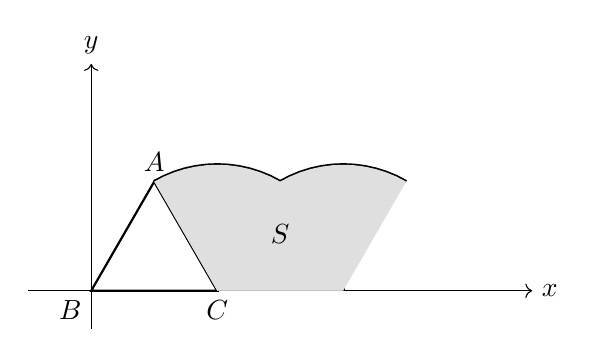
\begin{tikzpicture}[scale=1.6]
  % 軸
  \draw[->] (-0.5,0) -- (3.5,0) node[right] {$x$};
  \draw[->] (0,-0.3) -- (0,1.8) node[above] {$y$};
  % 初期三角形
  \draw[thick] (0,0) -- (1,0) -- (0.5,0.866) -- cycle;
  \node[below left] at (0,0) {$B$};
  \node[below] at (1,0) {$C$};
  \node[above] at (0.5,0.866) {$A$};
  % 弧1: C中心, A から
  \draw[very thick, domain=120:0] plot ({1+cos(\x)},{sin(\x)});
  % 弧2: (2,0)中心
  \draw[very thick, domain=180:60] plot ({2+cos(\x)},{sin(\x)});
  % 通過領域の塗り
  \begin{scope}
    \clip (0,0) rectangle (3.2,1.7);
    \fill[gray!25, domain=120:0] plot ({1+cos(\x)},{sin(\x)}) -- (1,0) -- cycle;
    \fill[gray!25, domain=180:60] plot ({2+cos(\x)},{sin(\x)}) -- (2,0) -- cycle;
  \end{scope}
  \node at (1.5,0.45) {$S$};
\end{tikzpicture}
\end{center}

\kaitohead
頂点 $A$ の軌跡は，点 $C(1,0)$ を中心とする半径 $1$，中心角 $\dfrac{2\pi}{3}$ の円弧と，
点 $(2,0)$ を中心とする半径 $1$，中心角 $\dfrac{2\pi}{3}$ の円弧からなる．

扇形 $2$ つ分の面積は
$$2 \cdot \frac{1}{2} \cdot 1^2 \cdot \frac{2\pi}{3} = \frac{2\pi}{3}$$

さらに，弧と $x$ 軸の間に正三角形 $1$ 枚分 $\dfrac{\sqrt{3}}{4}$ が２回現れるから，求める面積は
$$S = \frac{2\pi}{3} + 2 \cdot \frac{\sqrt{3}}{4} = \frac{2\pi}{3} + \frac{\sqrt{3}}{2}. \qquad \blacksquare$$

\end{document}
